\section{Convolutional Networks}
% \subsection*{CNN General Structure}


% \begin{itemize}
%   \item Convolutional networks consist of sparsely connected convolutional layers in place of fully-connected linear layers
%   \item Pooling layers perform spatial downsampling (typically typically reducing the dimensions from $H \times W$ to $H / 2 \times W / 2$
%   \item A fully-connected network at the end performs classification based on the extracted features
% \end{itemize}


% \begin{itemize}
%   \item Fully connected NNs have $O\left(K^{2} L\right)$ parameters: training requires a lot of data
%   \item Fully connected neural networks interpret an image as a flattened vector, disregarding the original spatial dependencies
% \end{itemize}


% \subsection*{Convolution}
$
x_{n, m}^{(1)}=\sum_{k, l} f_{k, l} \cdot x_{n-k, m-l}^{(0)}
$, ($f$ is the learnable filter)

% \begin{itemize}
%   \item We consider local filters: $f_{k, l} \neq 0$ for small values of $|k|$ and $|l|$
% \end{itemize}

% $\rightarrow x_{n, m}^{(1)}$ only depends on the value of $x^{(0)}$ close to $(n, m)$

% $\rightarrow f$ represents the learnable weights

\begin{itemize}
  \item Same filter at every position - weight sharing

  \item Translation equivariance :shifted input results in shifted output
  % \item  Convolution requires fewer parameters which are universal across different locations

\end{itemize}


% \subsection*{Handling of borders}
% - Zero padding: Add zeros to each side of the input's boundaries $\Rightarrow$ same dimension as the input

% - Valid padding: Perform the convolution only where the entire filter fits inside the original data $\Rightarrow$ smaller dimensions than the input

% \subsection*{Filter for Multi-Channel Convolution}

% \begin{itemize}
%   \item For multi-channel inputs, the filter has the same number of channels as the input
%   \item The filter channels and the bias are the learnable parameters of the filter
% \end{itemize}

% \subsection*{Multi-Channel Output from Multiple Filters}
% - It is common to use multiple filters. Each filter processes the input to produce a separate channel

% - Applying different filters to an input generates multiple output channels.

% \subsection*{Convolutional Layer}

% % \begin{wrapfigure}{r}{0.5\columnwidth} 
% %     \centering
% %     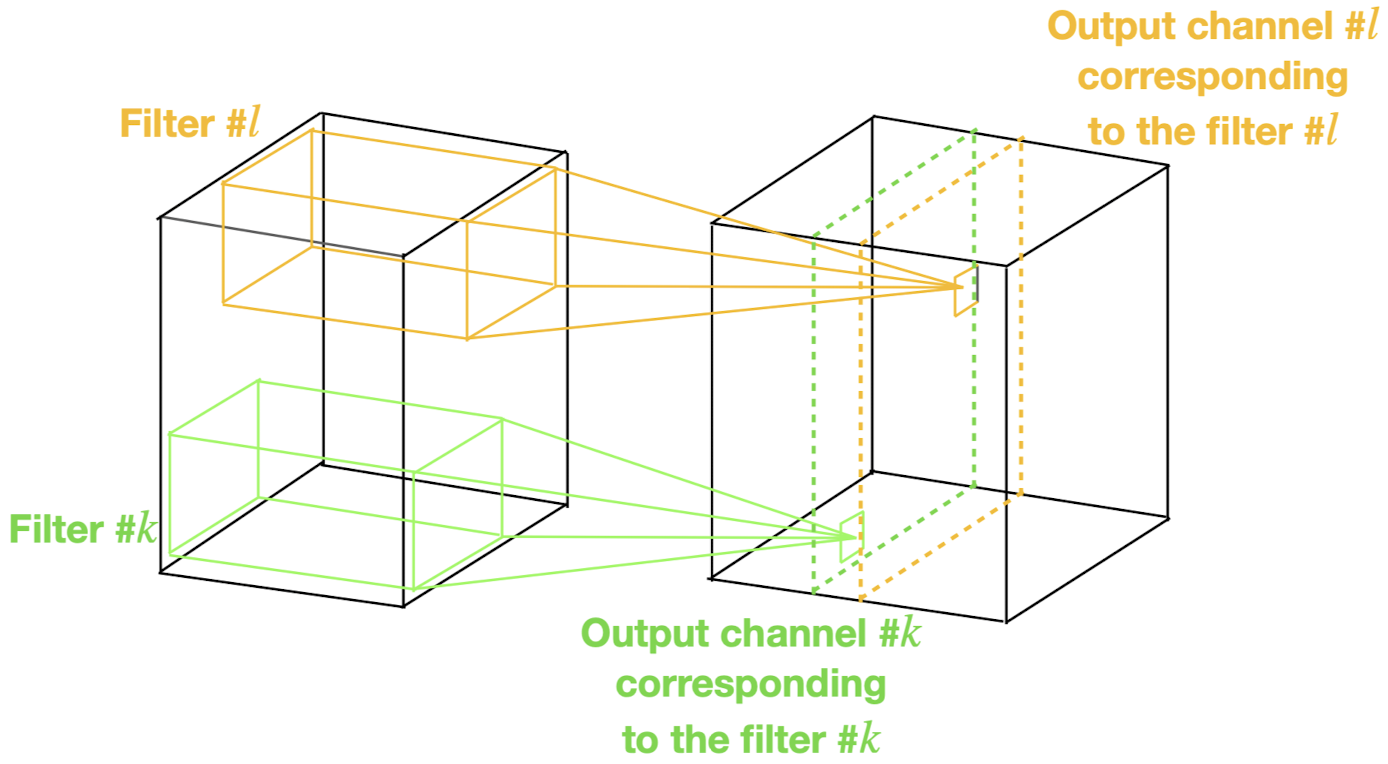
\includegraphics[width=0.5\columnwidth]{figures/conv_layer.png}
% %     \vspace{-10pt}
% % \end{wrapfigure}

% - A convolutional layer is composed of multiple filters

% - Each output channel corresponds to its own independent filter

% - Hyper-parameters of the convolutional layer: size, padding, stride


% \subsection*{Pooling}
% % - often applied after the convolutional layer

% - Max pooling: returns the maximum value of the portion of the convolved feature that is covered by the kernel

% - Average pooling: returns the average value of the portion of the convolved feature that is covered by the kernel

% - Pooling is a downsampling operation that reduces the spatial dimensions of the convolved feature

% - Remark: Pooling layers do not have learnable parameters 

% - Hyperparameters are the size, type, and stride of the pooling operation

% \subsection*{Non-linearity and CNNs}

% - Non-linearity such as ReLU is included after each convolutional layer to make the model non-linear

% \subsection*{CNNs: General Structure}
% % \includegraphics*[width=\columnwidth]{figures/CNN.jpg}

% - Depth: $\uparrow$ \# channels, $\downarrow$ dimensions

% - Receptive field increases with depth:

% \begin{itemize}
%   \item First layers extract low-level features, e.g., edges, colors ($\downarrow$ receptive field + $\downarrow$ depth)
%   \item Subsequent layers extract high-level features, e.g., objects ($\uparrow$ receptive field + $\uparrow$ depth)
% \end{itemize}

% - ConvNet reduces the images to a form easier to process without losing essential features

% \subsection*{Backpropagation with weight sharing}
% - Weight sharing is used in CNN: many edges use the same weights

\underline{Training:}

\begin{enumerate}
  \item Run backpropagation as if the weights were not shared

  \item Sum the gradients of all edges that share the same weight

\end{enumerate}

% Let $f(x, y, z): \mathbb{R}^{3} \rightarrow \mathbb{R}$ and $g(x, y)=f(x, y, x)$

% $
% (\frac{\partial g}{\partial x}(x, y), \frac{\partial g}{\partial y}(x, y)) \underset{\text {Chain rule }}{=}(\frac{\partial f}{\partial x}(x, y, x)+\frac{\partial f}{\partial z}(x, y, x), \frac{\partial f}{\partial y}(x, y, x))
% $

% \subsection*{Learned Convolutional Filters}

% - Edge and color detectors typically emerge when trained on large datasets

% - Individual Activations Can Be Interpretable

% - Activations in later layers detect more complex patterns

% \subsection*{Residual Networks}
% \subsection*{Skip Connections and Residuals}
% \begin{itemize}
%   \item Starting point: Adding more layers should lead to the same or lower training loss as they can learn the identity function

%   \item ResNet paper indicates that this is not always the case

%   \item Solution: add a skip connection around some layers $F(\mathbf{X})$

%   \item Standard network: $\mathbf{Y}=F(\mathbf{X})$

%   \item Residual network: $\mathbf{Y}=R(\mathbf{X})+\mathbf{X}$ where $R(\mathbf{X})$ is called a residual branch


%   \item Technical detail: If $\operatorname{size}(\mathbf{Y}) \neq \operatorname{size}(\mathbf{X})$, additional operations are needed on the skip connection to match the dimensions

%   \item Skip connections address the observed convergence issue, making the training of very deep networks (with hundreds of layers) feasible

%   \item Skip connections are used in almost all modern neural networks (including CNNs and transformers)

% \end{itemize}


% \subsection*{Popular architectures}

% VGG \& ResNet


% \subsection*{Data Augmentation}
% - Generate new data from the data

% - Note dangers of excessive augmentation (e.g. rotation on MNIST)!

% - Transformation $\tau: \mathbb{R}^{d} \rightarrow \mathbb{R}^{d}$ which preserves the labels (i.e., $y_{x}=y_{\tau(x)}$ )

% $
% S=S_{\text {train }} \cup\left\{\left(\tau\left(x_{i}\right), y_{i}\right)\right\}_{i=1}^{n}
% $

% \begin{itemize}
%   \item We train on more data

%   \item Encourages models to be invariant to $\tau$

%   \item It can be seen as regularization

%   \item These transformations are task and dataset specific

% \end{itemize}

% - Pictures can also be cropped, resized, or perturbed by a small amount of noise



\subsection*{Weight Decay: $l_{2}$-regularization}

- Regularize weights without bias:
$
\min \mathscr{L}+\frac{\lambda}{2} \sum_{l}\left\|\mathbf{W}^{(l)}\right\|_{F}^{2}
$

- Favors small w which can aid in generalization and opti

% - Optimization with gradient descent:

$
\left(w_{i, j}^{(l)}\right)_{t+1}=\left(w_{i, j}^{(l)}\right)_{t}-\eta \nabla \mathscr{L}-\eta \lambda\left(w_{i, j}^{(l)}\right)_{t}=\underbrace{(1-\eta \lambda)}_{\text {weight decay }}\left(w_{i, j}^{(l)}\right)_{t}-\eta \nabla \mathscr{L}
$

- Interaction with BatchNorm:

\begin{itemize}
  \item $\mathrm{BN}(\mathbf{W X})=\mathrm{BN}(\alpha \mathbf{W X})$ for $\alpha \in \mathbb{R}_{>0}$ (assuming $\varepsilon \approx 0$ )
  % \item $\mathrm{BN}$ is scale invariant in $\mathbf{W}$, hence there is no direct regularization effect from WD
  % \item However, the training dynamics differ 
\end{itemize}


% \subsection*{Dropout: randomly drop nodes}
% - Def: At each training step, retain with probability $p^{(l)}$ each node in layer $(l)$ :

% - We drop nodes independently for each element of a mini-batch

% - Training phase: Run one step of SGD on the subnetwork and update the weights

% - Testing phase: 

% \begin{itemize}
%     \item Use all nodes
%   \item Scale each of them by the factor $p^{(l)}$ to ensure that the expected output (when considering the probability of dropping nodes during training) matches the actual output at test time
% \end{itemize}

% - Remark: Weight rescaling can be implemented during training time by scaling the weights by $1 / p^{(l)}$ after each weight update - how it is implemented in practice

% - Note: Variance is generally not preserved and as a result Dropout often works poorly with normalization

% \subsection*{Dropout: results}
% \begin{itemize}
%   \item Setting: Fully-connected networks of different width and depth on MNIST

%   \item Dropout results in lower test error

%   \item However, dropout typically requires more iterations to converge due to increased stochastic noise

% \end{itemize}


% \subsection*{Recap}
% \begin{itemize}
%   \item Convolutional networks are composed of sparsely connected convolutional layers instead of fully-connected linear layers

%   \item The same convolution is applied as a sliding window across all spatial locations

%   \item Data augmentation usually results in a significant improvement in the model's generalization performance

%   \item Weight decay and dropout can further enhance the performance, though typically to a lesser extent

% \end{itemize}